\documentclass[lettersize,journal]{IEEEtran}
\usepackage{float}
\usepackage{amsmath,amsfonts}
%\usepackage{algorithmic}
\usepackage{algorithm}
\usepackage{algpseudocode}
\usepackage{array}
\usepackage[caption=false,font=normalsize,labelfont=sf,textfont=sf]{subfig}
\usepackage{textcomp}
\usepackage{stfloats}
\usepackage{url}
\usepackage{verbatim}
\usepackage{graphicx}
\usepackage{cite}

% clear in final version
\usepackage{xcolor}
\definecolor{highlightgreen}{rgb}{0.1, 0.6, 0.1} % A nice, readable dark green
% \definecolor{highlightgreen}{HTML}{009933} % Alternative definition
\newcommand{\greenhighlight}[1]{\textcolor{highlightgreen}{#1}}

\definecolor{deleteRed}{rgb}{0.8, 0, 0} % A noticeable red
\newcommand{\markfordelete}[1]{\textcolor{deleteRed}{#1}}
% Alternative: Just red, no strikethrough
% \newcommand{\markfordelete}[1]{\textcolor{deleteRed}{#1}}
%

\UseRawInputEncoding

\usepackage[colorlinks=true, linkcolor=blue, citecolor=blue]{hyperref}

\hyphenation{op-tical net-works semi-conduc-tor IEEE-Xplore}
\def\BibTeX{{\rm B\kern-.05em{\sc i\kern-.025em b}\kern-.08em
		T\kern-.1667em\lower.7ex\hbox{E}\kern-.125emX}}
\usepackage{balance}
\begin{document}
	\title{Density-Based Dynamic Ensemble Learning Algorithm via Gaussian Mixture Model Clustering for Enhanced Predictive Analytics.}
	\author{}
	
	\markboth{IEEE Transactions on Emerging Topics in Computational Intelligence, ~Vol.~XX, No.~YY, Month~Year.}%
	{Density-Based Dynamic Ensemble Learning Algorithm via Gaussian Mixture Model Clustering for Enhanced Predictive Analytics.}
	
	\maketitle
	\begin{abstract}
		 Dynamic ensemble learning is a powerful technique for enhancing predictive accuracy and robustness by combining multiple classifiers. However, traditional methods face challenges in providing personalized predictions and balancing classifier diversity with ensemble generalization.
		 This paper introduces a novel Density-Based Dynamic Ensemble Learning Algorithm using Gaussian Mixture Models to address these issues. The proposed algorithm leverages Gaussian Mixture Models to capture complex data structures, creating subsets that reflect specific patterns, which are then used to train distinct base classifiers, ensuring diversity within the ensemble. The density-based dynamic selection strategy intelligently selects classifiers for each test instance based on its proximity to these clustered subsets, enhancing accuracy and adaptability. The algorithm is evaluated against single ensemble methods as well as other dynamic ensemble methods to assess its performance and effectiveness, using logistic regression, support vector machine, k-nearest neighbors, and decision tree as base learners. Results demonstrate that the proposed method, particularly when combined with logistic regression and support vector machine, outperforms other methods, underscoring the effectiveness of the density-based selection strategy. Further analysis shows that increasing the number of clusters and sampling ratio improves the F-score, though with diminishing returns beyond a certain point.
	\end{abstract}
	
	\begin{IEEEkeywords}
		Dynamic Ensemble Learning, Gaussian Mixture Models, Density-Based Ensemble Learning, Predictive Analytics, Model Personalization, Decision-Making Efficiency.
	\end{IEEEkeywords}
	
	\section{Introduction}
	\IEEEPARstart{T}{he} advent of dynamic ensemble classifiers heralds a new epoch in machine learning, addressing critical needs across sectors such as medical diagnostics \cite{zimmerman_early_2019}, cybersecurity \cite{folino_ensemble_2016}, and more. Recent advancements have shown that these classifiers significantly enhance the accuracy and robustness of human activity recognition (HAR) systems, as well as medical diagnostics, particularly in fields like cardiovascular disease detection using novel ensemble classifiers \cite{hosseini_chagahi_cardiovascular_2024}. For instance, evolutionary dual-ensemble class imbalance learning methods have demonstrated superior performance in recognizing diverse human actions by optimizing the combination of base classifiers \cite{guo_evolutionary_2022}. Ensemble learning, by synergizing multiple classifiers, offers unparalleled robustness and accuracy, far surpassing the capabilities of individual classifiers \cite{xu_novel_2023, lv_classifier_2019, mao_end--end_2021, li_-network_2021, pari_multitier_2020}. 
	This approach, known as Multiple Classifier Systems (MCS), leverages diverse models for enhanced prediction reliability. Specifically, Dynamic Ensemble Selection (DES) refines this concept by customizing classifier combinations for each test instance, thus ensuring adaptability and precision in predictive analytics \cite{nguyen_ensemble_2020, zhang_distance-based_2019}. The sophistication of ensemble methods is evident in their application to complex tasks, where they have consistently outperformed single-model approaches \cite{zhao_experimental_2021, choi_ddes_2021}. Despite the advancements, ensemble learning faces significant challenges. Key among these is the need for personalized predictions for scenarios such as fluctuating market trends or evolving cybersecurity threats \cite{ditzler_learning_2015}. 
	Traditional ensemble methods struggle with the nuanced balance between classifier diversity and ensemble generalization, a barrier to harnessing their full potential \cite{lessmann_benchmarking_2015}. Furthermore, the dilemma of maintaining robustness without increasing ensemble complexity presents a persistent challenge in dynamic selection methods. These issues underscore the necessity for innovative solutions that can adapt to variable data conditions while maintaining accuracy and efficiency \cite{ditzler_learning_2015}.
	
	Our proposed model, the Density-Based Dynamic Ensemble Learning algorithm via Gaussian Mixture Model clustering (DDEL-GMM), addresses these challenges with a groundbreaking approach in dynamic ensemble learning. By integrating Gaussian Mixture Models (GMM) for sophisticated data clustering and a density-based dynamic selection strategy, DDEL-GMM enhances personalization and accuracy in prediction tasks. Specifically, it is designed to adapt to complex data structures and enhance predictive personalization, which are common hurdles in traditional ensemble methods. By advancing beyond these limitations, DDEL-GMM sets a new standard for adaptability, precision, and decision-making efficiency in the field. This model does not merely improve existing methods; it represents a paradigm shift in how ensemble learning can be approached, promising significant advancements in various complex and dynamic scenarios.
	
	This study leverages a complex dataset with high-dimensional characteristics, generated from wearable sensor technology, to rigorously evaluate the performance of the proposed dynamic ensemble learning model. The dataset originates from recordings of human activity, captured using accelerometers and gyroscopes integrated into smartphones. These sensors meticulously track the subtle movements and changes in orientation as subjects engage in various physical activities, providing a rich source of information for activity recognition tasks.
	
	Each recording in the dataset corresponds to a distinct activity performed by a subject and encapsulates a time series of sensor readings. At each time step within a recording, the accelerometers and gyroscopes measure linear acceleration and angular velocity, respectively, across three orthogonal axes (X, Y, and Z). This intricate sampling process generates a high-dimensional feature space, where each feature represents the magnitude of a specific sensor measurement (acceleration or angular velocity) along a particular axis at a given time instance. To address the computational challenges of this high-dimensional space and to ensure model stability, Principal Component Analysis (PCA) was applied as a preprocessing step. The analysis showed that retaining 157 principal components was sufficient to preserve 95\% of the variance, enabling efficient and effective clustering and classification within the DDEL-GMM framework.
	
	The raw sensor data, while rich in information, is inherently prone to noise and uncertainty. This stems from a confluence of factors inherent to the nature of wearable sensing: 
	
	\begin{itemize}
		\item \textbf{Sensor Imperfections:} Like all physical instruments, accelerometers and gyroscopes exhibit limitations in their sensitivity and accuracy. Minute variations in sensor readings can arise from internal electronic noise, temperature fluctuations, and manufacturing inconsistencies. 
		\item \textbf{Environmental Interference:} The surrounding environment can introduce spurious signals that contaminate the sensor readings. Electromagnetic interference from nearby electronic devices, vibrations from the floor or other surfaces, and even changes in air pressure can all contribute to noise in the data. 
		\item \textbf{Placement and Movement Variability:} The placement of the smartphone on the subject's body (e.g., pocket, belt, hand) and variations in the manner of movement can significantly influence the sensor readings. Slight shifts in the device's position or changes in the execution of an activity introduce inconsistencies into the collected data. 
	\end{itemize}

	These inherent challenges, particularly the variability arising from sensor placement and individual movement styles, underscore the limitations of a rigid, single model classification model.
	 This is where the proposed dynamic ensemble model demonstrates its strength. By employing Gaussian Mixture Models (GMMs), the model effectively captures the underlying data distribution, accounting for its multi-modality and effectively distinguishing meaningful patterns from random fluctuations. Moreover, the model’s density-based selection strategy ensures that for each test instance, the most appropriate base learners, trained on relevant data partitions, are selected for prediction. This dynamic and context-aware approach enhances the model's robustness and accuracy, enabling it to achieve high performance even when faced with the complexities of real-world sensor data.
	
	\greenhighlight{
		This paper is organized as follows: 
		Section II provides a comprehensive review of existing literature in ensemble learning, dynamic ensemble selection, and related clustering approaches, positioning our work within this context, highlighting the challenges addressed, and underscoring its contributions. Section III details the proposed DDEL-GMM framework, elaborating on the GMM-based data clustering and the density-based dynamic selection mechanism. Section IV presents the experimental setup, discusses the evaluation results comparing DDEL-GMM with other methods, and analyzes the impact of key parameters. Finally, Section V concludes the paper, summarizing the findings and suggesting potential directions for future research.
	}

\section{Literature Review}
\greenhighlight{While ensemble learning and dynamic ensemble selection (DES) have shown considerable promise \cite{nguyen_ensemble_2020, zhang_distance-based_2019, cruz_dynamic_2018}, significant challenges remain, particularly in effectively handling complex data distributions, adapting predictions to individual instances, and efficiently balancing classifier diversity with generalization \cite{ditzler_learning_2015, lessmann_benchmarking_2015}. This review examines existing approaches and positions our proposed DDEL-GMM, which addresses these challenges through a novel density-based framework leveraging Gaussian Mixture Models, by highlighting its differences from state-of-the-art methods and underscoring its contributions.}

\subsection{Ensemble Learning and Dynamic Ensemble Selection}
\noindent Ensemble learning marks a significant stride in machine learning, particularly in the context of predictive modeling. Combining multiple models, such as through Bagging, Random Subspace Method, and Random Forest, ensemble learning approaches have improved predictive accuracy and robustness \cite{cruz_dynamic_2018}. The diversification among base models is key to the success of these methods. Furthermore, dynamic ensemble selection techniques have evolved, allowing for the adaptation of model selection based on each test sample's specific characteristics, thereby offering more personalized predictions \cite{ko_dynamic_2008}. This is particularly useful in applications like breast cancer detection, where an ensemble of deep learning networks has been shown to improve diagnostic accuracy using consensus-adaptive weighting techniques \cite{dehghan_rouzi_breast_2023}. 

The DeepCluE approach employs a convolutional neural network to generate diverse clusterings from multiple layers, effectively selecting the most informative ones for final clustering \cite{huang_deepclue_2023}. Similarly, the probabilistic combination of non-linear eigenprojections for ensemble classification enhances the reliability of classifications by integrating a probabilistic support vector machine (SVM) approach, allowing for better handling of uncertainty in predictions \cite{arco_probabilistic_2023}.

\greenhighlight{These examples illustrate the ongoing efforts to enhance ensemble methods, yet many still grapple with optimal diversity generation and adaptive selection in highly heterogeneous data. Our DDEL-GMM contributes by proposing a GMM-based data partitioning that aims to create inherently diverse and specialized base classifiers, followed by a density-based selection mechanism that adapts to local data characteristics more fluidly than some consensus or static weighting schemes.}

\subsection{Ensemble Pruning and Clustering-based Approaches}
\noindent Ensemble pruning optimizes the selection of classifiers within an ensemble to balance efficiency and performance. Diverse strategies, including ranking-based methods and optimization-based methods like Optimum-Path Forest (OPF) ensemble pruning \cite{fernandes_pruning_2017}, illustrate the evolving landscape of ensemble pruning. Additionally, clustering-based approaches, which organize similar classifiers and select the most representative ones for the ensemble, add another dimension to enhancing the efficiency of ensemble learning systems \cite{cruz_dynamic_2018}.

\greenhighlight{While pruning focuses on selecting from an existing pool, and traditional clustering often groups classifiers post-training, DDEL-GMM integrates clustering directly into the training data partitioning phase using GMMs. This proactive approach aims to build a diverse and competent ensemble from the outset, rather than pruning less effective members later, addressing the challenge of efficiently constructing high-performing ensembles. The contribution here is a more integrated clustering-for-diversity strategy rather than clustering-for-pruning.}

\subsection{Dynamic Classifier Selection Techniques}
\noindent Dynamic classifier selection techniques, focusing on estimating and utilizing the competence levels of classifiers, have seen significant advancements. Approaches like META-DES and Dynamic Selection on Complexity (DSOC) have emphasized the importance of the region of competence in classifier selection, leading to more accurate and tailored predictions. The refinement of these techniques, considering both correctly-classified and misclassified samples, has contributed to improved accuracy in dynamic selection systems, making them more effective in diverse machine learning applications \cite{cruz_dynamic_2018}.

\greenhighlight{Many DES techniques define the region of competence based on K-Nearest Neighbors or local instance similarity. DDEL-GMM defines competence based on the probability density of a test instance with respect to GMM-defined clusters. This is a key difference, as it moves from instance-based distance to a probabilistic, model-based density estimation for competence assessment, potentially offering more robust selections in sparse or noisy regions. The contribution is a density-informed competence estimation for DES.}

\subsection{Recent Advancements and Current Limitations}
\noindent Guo et al. \cite{guo_dynamic_2021} exposed the shortcomings of traditional scoring systems like SAPS II, SOFA \cite{tekin_comparison_2024}, and single machine learning models in critical care settings \cite{sagi_ensemble_2018}. This work introduced the Dynamic Ensemble Learning Algorithm based on K-means (DELAK) method, employing K-means sampling and dynamic ensemble selection to address these issues, an approach in line with current trends in ensemble methods for enhanced predictive performance \cite{dong_survey_2020, jiang_clustering-based_2019}. However, DELAK, like many other distance-based dynamic ensemble methods, struggled to capture the intricacies of complex data distributions and personalize predictions for new test instances, a limitation echoed in contemporary research \cite{mienye_survey_2022, gonzalez_practical_2020}. 

\greenhighlight{DELAK's reliance on K-means, which typically forms spherical clusters and can be sensitive to initialization, is a key point of divergence for DDEL-GMM. Our approach uses GMMs, which can model non-spherical clusters and provide a probabilistic assignment, addressing the challenge of representing complex data distributions more accurately. The contribution of DDEL-GMM here is the use of a more flexible clustering algorithm (GMM) to better partition complex data spaces for training specialized classifiers, leading to improved personalization.}

Further contributions, such as the META-DES.Oracle framework in \cite{cruz_meta-oracle_2017}, extended the scope by utilizing meta-learning for classifier selection. While groundbreaking, this approach grappled with potential overfitting and computational complexities stemming from its intricate meta-feature framework and the optimization process using PSO-BP optimization algorithm, which integrates Particle Swarm Optimization (PSO) with the Backpropagation (BP) neural network training method \cite{al-andoli_ensemble-based_2023}. Additionally, its reliance on linear classifiers limited its effectiveness in scenarios with non-linear relationships. \greenhighlight{DDEL-GMM, in contrast, does not employ a meta-learning layer for selection but rather a direct density-based assessment, potentially reducing complexity and overhead compared to intricate meta-feature frameworks. It also inherently supports non-linear base classifiers without modification to the selection mechanism itself, addressing the challenge of applicability to diverse base models.} Recent ensemble learning advancements have focused on overcoming these limitations by exploring diverse methods like bagging, boosting, and decision tree ensembles, which have been shown to offer more robust solutions in handling complex data patterns \cite{sagi_ensemble_2018}. These techniques, along with novel approaches such as ensemble methods for dirty data, provide a framework for integrating multiple learning algorithms and addressing the challenges observed in META-DES.Oracle, particularly ensuring model generalization \cite{liu_ensemble_2023}.

Similarly, Wang et al. \cite{wang_ensemble_2021} and Zhang et al. \cite{zhang_distance-based_2019} introduced novel selection methods, yet faced challenges in the sensitivity of unsupervised ensemble selection to the influence of class labels and the limitations of distance metrics for assessing classifier competence. These issues are also reflected in studies focusing on unsupervised data selection and ensemble classifiers, which further emphasize the complexities in selecting and combining multiple learning models without the guidance of labeled data \cite{huang_ensemble_2016}. \greenhighlight{To address such challenges related to unsupervised selection and reliance on distance metrics, DDEL-GMM employs a distinct strategy. It leverages GMM-identified data structures to inform the creation of specialized base learners from labeled data and subsequently uses a density-based mechanism for dynamic classifier selection. This approach aims to provide a more robust competence assessment by moving beyond simple distance metrics and more effectively incorporating insights from the underlying data distribution, even when initial structures are found unsupervisedly, thereby offering an alternative to the sensitivities noted in prior works.} Recent advancements in unsupervised ensemble classification, particularly in handling data dependencies and using clustering ensembles for feature selection, provide new perspectives and potential solutions to these challenges \cite{tian_improved_2022}, \cite{traganitis_unsupervised_2022, ayerdi_spatially_2015}.

B. et al. \cite{b_data_2023} tackled the issue of class overlapping and noise, highlighting the inadequacy of existing ensemble methods in handling these complexities. Additionally, Perez-Gallego et al. \cite{perez-gallego_dynamic_2019} addressed the unique challenges in quantification tasks, proposing a dynamic ensemble method integrating data complexity measures. However, adaptability to data variability data environments remained a challenge for these approaches, an issue further explored in recent works such as \cite{alam_dynamic_2020} dynamic neural network ensemble algorithm, which effectively balances diversity and accuracy across various inputs. New insights into dynamic ensemble methods for data streams are provided by \cite{gomes_survey_2017}, who discuss the integration of drift detection algorithms and dynamic updates, crucial for real-time data processing. \greenhighlight{The GMM component of DDEL-GMM is inherently suited to model overlapping distributions through probabilistic assignments, and the density-based selection is designed to be adaptive. This addresses the challenge of handling class overlap more effectively than methods relying on hard partitioning, as the probabilistic nature of GMMs can model these overlapping regions. The contribution is enhanced robustness in scenarios with significant class overlap.}

Yet, it encountered difficulties in handling highly complex data distributions, particularly in defining regions of competence and adapting to significant data variation \cite{sierra_k_2011}. The challenges of adaptability in dynamically changing data environments are also addressed in the META-DES framework, which employs meta-learning techniques to enhance classifier competence through a variety of meta-features \cite{gomes_survey_2017}. Additionally, the dynamic ensemble selection for quantification tasks, which further pushes the boundary of dynamic adaptability using data complexity measures, shows promising results in specific applications such as agricultural yield prediction and financial forecasting \cite{perez-gallego_dynamic_2019, swaminathan_meta_2022}. 

\greenhighlight{In summary, while existing dynamic ensemble methods like K-means-based (e.g., DELAK) and meta-learning based (e.g., META-DES.Oracle) have advanced the field, they often face limitations in handling highly complex and overlapping data distributions, potential computational overhead, or sensitivity to the geometric definition of competence regions. Our proposed DDEL-GMM differentiates itself by integrating Gaussian Mixture Models for sophisticated data clustering—capturing multi-modal and non-spherical data patterns—and a subsequent density-based dynamic selection strategy. This approach directly addresses the challenges of achieving robust personalization and adaptability in complex, noisy environments. The primary contribution of DDEL-GMM to the literature is thus a more flexible and statistically grounded framework for dynamic ensemble learning, designed to improve predictive accuracy and decision-making efficiency by more accurately modeling data sub-structures and employing a nuanced, density-informed mechanism for classifier selection, especially for data exhibiting intricate structures, as often encountered in real-world applications like sensor-based activity recognition.}
	\section{Methodology}
	
	\subsection{The proposed DDEL-GMM framework}
	
	\noindent This paper proposes a novel dynamic ensemble model, the Density-Based Dynamic Ensemble Learning algorithm via Gaussian Mixture Model clustering (DDEL-GMM). \greenhighlight{DDEL-GMM is designed to enhance predictive accuracy in providing personalized predictions.} By employing Gaussian Mixture Models (GMM) for clustering and a density-based decision-making approach, \greenhighlight{the model aims to achieve} a more granular analysis of complex data distributions and \greenhighlight{provide} a robust framework for classifier competence estimation.
	
	As illustrated in Figure \ref{fig:training_phase_diagram}, the training phase of \greenhighlight{DDEL-GMM} involves leveraging GMM to effectively capture the underlying structure of the data. This approach facilitates the creation of specialized classifiers that are adept at recognizing specific data patterns within complex and overlapping distributions.
	Furthermore, as depicted in Figure \ref{fig:generalization_phase_diagram}, the generalization phase employs a density-based dynamic ensemble selection mechanism. This ensures that, during prediction, the most relevant classifiers contribute more significantly based on the density estimation of the input data point, thereby enhancing the model's overall performance and robustness.
	
	\begin{figure*}[!t]
		\centering
		%\vspace{5cm}  % Add 1cm of space above the figure
		
\includegraphics[width=0.9\linewidth]{training_phase_diagram}
		%
\includegraphics[width=2.5in]{training_phase_diagram}
		\caption{Training phase of proposed model}
		\label{fig:training_phase_diagram}
	\end{figure*}
	
	Furthermore, as depicted in Figure \ref{fig:generalization_phase_diagram}, the generalization phase employs a density-based dynamic ensemble selection mechanism. This ensures that, during prediction, the most relevant classifiers contribute more significantly based on the density estimation of the input data point, thereby enhancing the model's overall performance and robustness.
	
	\begin{figure*}[!t]
		\centering
		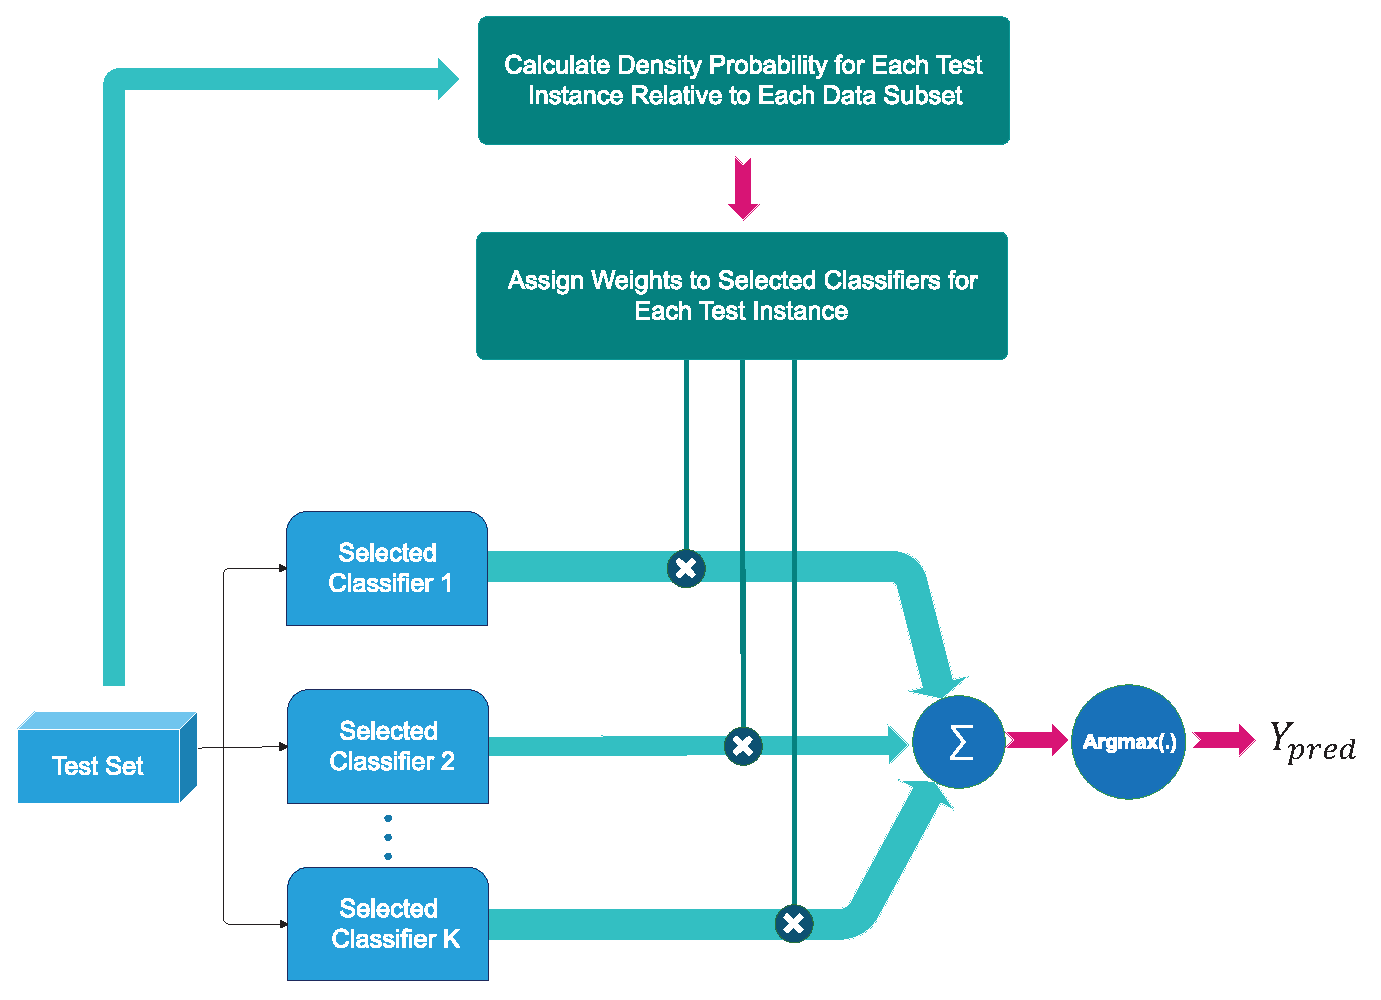
\includegraphics[width=0.9\linewidth]{generalization_phase_diagram}
		\caption{Generalization phase of proposed model}
		\label{fig:generalization_phase_diagram}
	\end{figure*}
	
	Significant contributions in the realm of GMM for ensemble learning include \cite{li_gaussian_2018}'s work on Gaussian mixture learning, which improves the efficiency and accuracy of ensemble models real-world applications by combining hierarchical clustering with the Expectation-Maximization algorithm. Additionally, Liu et al.'s \cite{liu_robustly_2023} recent work on robustly learning mixtures of Gaussians provides theoretical backing for the efficacy of GMM in complex distribution scenarios, supporting our model's approach. This approach allows our model to excel in scenarios where data patterns are intricate and where adaptability to changing data distributions is crucial. By effectively capturing the nuances of complex data and dynamically weighting the contributions of individual classifiers, our model offers a significant advancement in the field of ensemble learning.
	
	We introduce an advanced ensemble learning strategy that is deeply rooted
	in the principles of data density and specialization. Our proposed methodology consists of two interrelated components: the Gaussian Mixture Model
	(GMM) Sampling and the Density-based Dynamic Ensemble.
	
	\subsection{GMM Clustering \& Sampling}
	\noindent Traditional ensemble techniques often create subsets of data either randomly or using simple heuristics. While effective for many datasets, the
	increasing complexity and multimodal nature of modern datasets necessitate
	a more sophisticated approach. Enter GMM Sampling, a method designed to capture the intricate structures within datasets
	and thereby enhance the versatility of ensemble models.
	
	\textbf{Motivation:} The driving force behind employing GMM in the ensemble paradigm is its ability to recognize and capture underlying patterns
	within datasets. Given that many datasets exhibit a multimodal distribution,
	GMM’s capability to model data as a mixture of several Gaussian distributions becomes invaluable. By ensuring that each base classifier in the ensemble is trained on data that mirrors these Gaussian components, we bolster
	the ensemble’s capacity to recognize and respond to subtle data structures.
	
	\textbf{GMM Overview:}
	Mathematically, a Gaussian Mixture Model represents data as a weighted combination of M Gaussian distributions as shown in Equation \ref{eq:Gaussian-distributions1}.
	
	\begin{equation}
		\label{eq:Gaussian-distributions1}
		p(\mathbf{x})=\sum_{i=1}^M \pi_i \mathcal{N}\left(\mathbf{x} \mid \mu_i, \Sigma_i\right)
	\end{equation}
	
	Where:
	\begin{itemize}
		\item $x$ is a data point.
		\item $\pi_i$ denotes the mixture weight of the $i^{{th }}$ Gaussian.
		\item $\mathcal{N}\left(\mathbf{x} \mid \mu_i, \Sigma_i\right)$ is the Gaussian distribution with parameters mean $\mu_i$ and covariance ${\Sigma}_i$.
	\end{itemize}
	
	The Gaussian distribution $\mathcal{N}\left(\mathbf{x} \mid \mu_i, {\Sigma}_i\right)$ is defined as shown in Equation \ref{eq:Gaussian-distributions2}:
	
	\begin{equation}
		\label{eq:Gaussian-distributions2}
		\mathcal{N}\left(\mathbf{x} \mid \mu_i, {\Sigma}_i\right) = 
		\begin{aligned}[t]
			&\frac{1}{(2 \pi)^{d / 2}\left|{\Sigma}_i\right|^{1 / 2}} \\
			&\times \exp \left(-\frac{1}{2}\left(\mathbf{x}-\mu_i\right)^T {\Sigma}_i^{-1}\left(\mathbf{x}-\mu_i\right)\right)
		\end{aligned}
	\end{equation}
	
	
	where d is the dimensionality of $x$.
	
	\textbf{Parameter Estimation via Expectation-Maximization (E-M):}
	The crux of GMM lies in the accurate estimation of its parameters. The E-M algorithm serves this purpose. It’s an iterative algorithm, progressively refining
	the parameters to maximize the likelihood of observing the given data:
	
	\begin{enumerate}
		\item \textbf{E-Step:} Computes the posterior probabilities, essentially estimating the likelihood of a data point originating from a specific Gaussian component. 
		\begin{equation}\label{eq:E-Step}
			\gamma_{ji} = \frac{\pi_i \mathcal{N}(x_j | \mu_i, \Sigma_i)}{\sum_{k=1}^{K} \pi_k \mathcal{N}(x_j | \mu_k, \Sigma_k)} \quad \text{for } i = 1, 2, \dots, K
		\end{equation}
		\item \textbf{M-Step:} Refines the parameters based on the probabilities obtained from the E-Step, ensuring that the overall likelihood of the data given the model parameters is maximized.
	\end{enumerate}
	
	The objective function $Q$ that the E-M algorithm aims to maximize is
	given by Equation \ref{eq:E-M-algorithm}.
	
	\begin{equation}\label{eq:E-M-algorithm}
		Q\left(\theta \mid \theta^{(t)}\right)=\sum_{i=1}^N \sum_{j=1}^M \gamma_{i j}^{(t)}\left[\log \pi_j+\log \mathcal{N}\left(\mathbf{x}_i \mid \mu_j, \mathbf{\Sigma}_j\right)\right]
	\end{equation}
	
	where $\gamma_{i j}^{(t)}$ is the posterior probability of the $i^{t h}$ data point belonging to the $j^{{th }}$ Gaussian component at iteration $t$.
	
	The update equations for the M-step are in Equations \ref{eq:M-step-1} to \ref{eq:M-step-3}.
	
	\begin{align}\label{eq:M-step-1}
		\pi_j^{(t+1)}=\frac{1}{N} \sum_{i=1}^N \gamma_{i j}^{(t)}
	\end{align}
	\begin{align}\label{eq:M-step-2}
		\mu_j^{(t+1)}=\frac{\sum_{i=1}^N \gamma_{i j}^{(t)} \mathbf{x}_i}{\sum_{i=1}^N \gamma_{i j}^{(t)}}
	\end{align}
	\begin{align}\label{eq:M-step-3}
		\mathbf{\Sigma}_j^{(t+1)}=\frac{\sum_{i=1}^N \gamma_{i j}^{(t)}\left(\mathbf{x}_i-\mu_j^{(t+1)}\right)\left(\mathbf{x}_i-\mu_j^{(t+1)}\right)^T}{\sum_{i=1}^N \gamma_{i j}^{(t)}} 
	\end{align}
	
	\textbf{Implications of GMM Sampling in Ensemble Learning:} Once the
	GMM parameters are derived, they play a pivotal role in segmenting the data.
	Each Gaussian component identified by the GMM provides insights into a
	specific data structure or pattern. When data points are assigned to subsets
	based on their association with these Gaussian components, it ensures that
	each subset is representative of a distinct data pattern. Training individual
	classifiers on these subsets equips the ensemble with a diverse set of experts,
	each attuned to a specific data structure. This nuanced approach to data sampling offers several advantages:
	\begin{itemize}
		\item \textbf{Diversity:} Ensures that base classifiers capture diverse perspectives of the data.
		\item \textbf{Specialization:} Each base classifier becomes an expert in a specific
		data pattern, enhancing the ensemble’s overall competence
		\item \textbf{Robustness:} By training specialized classifiers on distinct data patterns identified by GMM, the ensemble becomes more resilient to wide variations in the data, as no single classifier is overwhelmed by the entire dataset's complexity.
	\end{itemize}
	\textbf{Operational Steps:} With the GMM parameters in place, the methodology involves ranking data points based on their likelihoods under each
	Gaussian component. A sampling ratio, $phi$, then determines the fraction of
	top-ranking data points to be included in each subset. These subsets, rich in
	structure and pattern, serve as the training data for individual base classifiers.
	The detailed algorithmic steps for this process are outlined in Algorithm~\ref{algo:gmm}.
	
	\begin{algorithm}[!t]
		\caption{GMM Sampling}
		\label{algo:gmm}
		\textbf{Input:} Sampling ratio $\phi$; Training dataset $D$; Training data without labels $X$; Cluster number $K$ \\
		\textbf{Output:} Data subsets $D' = D'_1 \cup D'_2 \cup \dots \cup D'_K$
		\begin{algorithmic}[1]
			\Procedure{GMM Sampling}{$\phi$, $X$, $K$}
			\State Initialize $K$ Gaussian components with means \\
			$\mu_1, \mu_2, \dots, \mu_K$ and covariances $\Sigma_1, \Sigma_2, \dots, \Sigma_K$
			\State Initialize mixing coefficients $\pi_1, \pi_2, \dots, \pi_K$ such that $\sum_{i=1}^{K} \pi_i = 1$
			\Repeat
			\State \textbf{E-step:} Compute the responsibilities for each sample $x_j \in X$ using Equation \ref{eq:E-Step}.
			\State \textbf{M-step:} Update $\mu_m$, $\Sigma_m$, $\pi_m$ using Equations \ref{eq:M-step-1}, \ref{eq:M-step-2}, and \ref{eq:M-step-3}.
			\Until{convergence of parameters $\mu_i$, $\Sigma_i$, and $\pi_i$}
			\For{$i = 1, 2, \dots, K$}
			\State Compute the responsibilities for each instance in $X$ with respect to Gaussian component $i$
			\State Select $\text{int}(m \times \phi)$ instances with the highest responsibilities into partition $C'_i$
			\EndFor
			\State Return the labels in $D$ to instances in $C'$ to get $K$ data subsets $D' = D'_1 \cup D'_2 \cup \dots \cup D'_K$
			\EndProcedure
		\end{algorithmic}
	\end{algorithm}
	
	\subsection{Density-based Dynamic Ensemble Algorithm}
	\noindent Traditional ensemble learning methods often rely on the simple aggregation of base classifiers’ outputs, without considering the inherent nuances
	associated with the data regions that different base classifiers might be specialized in. The Density-based Dynamic Ensemble methodology emerges
	as an innovative response to this limitation, ensuring that the ensemble’s
	predictions are sensitive to the intrinsic data densities associated with test
	instances.
	
	\textbf{Motivation:} In fact, the base classifiers are in competition, and their contribution to the final decision depends on the density probability of the test instance relative to the data subset each classifier was trained on. Given that different data subsets (derived from Gaussian Mixture Model (GMM) sampling) capture unique data structures, the classifiers trained on these subsets specialize in different regions of the data distribution. Therefore, for any given test instance, it is essential to evaluate the competence of each classifier based on the density of the test instance within the relevant data subset, allowing the ensemble to leverage the classifiers with the highest competence.
	
	\textbf{Density Estimation:} The density of a test instance with respect to a data subset is indicative of the likelihood that the test instance belongs to that subset. Mathematically, the density $\rho_i(z)$ of a test instance $z$ concerning a subset $D_i^{\prime}$ is calculated using the Gaussian density function as shown in Equation \ref{eq: Density-Estimation}:
	\begin{equation}\label{eq: Density-Estimation}
		\rho_i(z)=\frac{1}{(2 \pi)^{\frac{d}{2}}\left|\Sigma_i\right|^{\frac{1}{2}}} \exp \left(-\frac{1}{2}\left(z-\mu_i\right)^T \Sigma_i^{-1}\left(z-\mu_i\right)\right)
	\end{equation}
	
	Where $\mu_i$ and $\Sigma_i$ are the mean and covariance matrix, respectively, of the Gaussian component associated with subset $D_i^{\prime}$.
	\textbf{Classifier Invocation:} After computing densities, the weight of each classifier is determined based on the density of the test instance with respect to the subset the classifier was trained on. This means that all classifiers contribute to the final prediction, but their influence is modulated by how well the test instance aligns with the data distribution of the corresponding subset. The weights are proportional to the densities, giving more importance to classifiers associated with higher densities for the test instance.
	
	\textbf{Decision Aggregation:} An ensemble's strength lies in its ability to amalgamate insights from multiple base classifiers. In the Density-based Dynamic Ensemble approach, predictions from all base classifiers are aggregated using a weighted voting scheme. Specifically, the probability vector for each class is calculated by weighting the predictions of each classifier according to the density of the test instance with respect to the subset on which that classifier was trained. The final predicted class label is the one with the highest combined probability. The algorithmic steps for this methodology are presented in Algorithm \ref{algo:density-based-dynamic-ensemble}.
	\begin{equation}
		y_{\text{pred}} = \operatorname{argmax}\left(\mathbf{y}_{\text{prob}}\right)
	\end{equation}
	Where $\mathbf{y}_{\text{prob}}$ is the probability vector of the test instance belonging to each class.
	
	\begin{algorithm}[H]
		\caption{The density-based dynamic ensemble for multi-class classification.}
		\label{algo:density-based-dynamic-ensemble}
		\begin{algorithmic}[1]
			\Require Training dataset $D' = D'_1 \cup D'_2 \cup \dots \cup D'_K$; Test example $e_i = (e_i^1, e_i^2, \dots, e_i^n)^T$; Gaussian components $\mu = \{\mu_i | i = 1, 2, \dots, K\}$ and $\Sigma = \{\Sigma_i | i = 1, 2, \dots, K\}$.
			\Ensure Predicted class label $y_{\text{pred}}$; Predicted probability vector $\mathbf{y}_{\text{prob}}$.
			\Procedure{Base Classifiers Training}{$D'$}
			\For{$\eta = 1, 2, \dots, K$}
			\State Train base model $h_\eta(\cdot)$ on training data subset $D'_\eta$
			\EndFor
			\State \textbf{Return} $h = \{h_\eta(\cdot) | \eta = 1, 2, \dots, K\}$
			\EndProcedure
			\Procedure{Ensemble}{$e_i, \mu, \Sigma, h$}
			\State Use each base classifier to predict the label of $e_i$ to get a result vector $\mathbf{h}(e_i) = (h_1(e_i), h_2(e_i), \dots, h_K(e_i))^T$
			\State Compute the density of test example $e_i$ with respect to each subset $D_i^{\prime}$ using the Gaussian density function:
			\begin{equation*}
				\rho_i(e_i) = \frac{1}{(2 \pi)^{\frac{d}{2}} |\Sigma_i|^{\frac{1}{2}}} \exp \left(-\frac{1}{2}(e_i-\mu_i)^T \Sigma_i^{-1} (e_i-\mu_i)\right)
			\end{equation*}
			\State Compute the weight vector for test example $e_i$: $\mathbf{w}_i = \left(\frac{\rho_1(e_i)}{\sum_{j=1}^{K} \rho_j(e_i)}, \frac{\rho_2(e_i)}{\sum_{j=1}^{K} \rho_j(e_i)}, \dots, \frac{\rho_K(e_i)}{\sum_{j=1}^{K} \rho_j(e_i)}\right)^T$
			\State Compute the probability vector of $e_i$ belonging to each class: $\mathbf{y}_{\text{prob}} = \mathbf{w}_i^T \cdot \mathbf{h}(e_i)$
			\State Assign the predicted class label:\\
			$y_{\text{pred}} = \arg\max(\mathbf{y}_{\text{prob}})$
			\EndProcedure
		\end{algorithmic}
	\end{algorithm}
	
	\textbf{Implications:} The Density-based Dynamic Ensemble approach offers several advantages:
	
	\begin{itemize}
		\item \textbf{Precision:} By considering data densities, the methodology ensures that all classifiers are considered, but the most relevant ones are given greater weight, enhancing classification precision.
		\item \textbf{Adaptability:} The approach is inherently adaptable, adjusting the ensemble’s response based on the test instance’s location within the data distribution.
		\item \textbf{Reduced Overfitting:} Leveraging density information ensures that the ensemble doesn’t overly rely on any single classifier, reducing the chances of overfitting.
	\end{itemize}
	In summation, the Density-based Dynamic Ensemble methodology infuses ensemble learning with a level of sensitivity and adaptability, ensuring that predictions are both accurate and attuned to the intricacies of the
	dataset’s distribution.
	
	\section{Results and Analysis}
	
	\noindent To evaluate the effectiveness of the four ensemble methods, this study employs several key performance metrics. The primary metric for assessing classification performance is the \textbf{F-score}, which provides a balanced measure of precision and recall. To understand the consistency and robustness of the methods, the \textbf{mean}, \textbf{standard deviation}, and \textbf{maximum} of the F-scores obtained from cross-validation are also reported. These metrics collectively offer a comprehensive view of each model's accuracy, stability, and peak performance.
	
	\noindent The performance of various ensemble methods, with a base learner count $nc = 6$ and a regularization parameter $\phi = 0.5$, is systematically compared in Table 1. This table assesses four ensemble methods—DensityE (a density-based ensemble method), DistE (a distance-based ensemble method), AvgE (an average-based ensemble method), and MaxE (a maximum-based ensemble method)—using four distinct types of base learners: logistic regression (lr), support vector machine (svm), k-nearest neighbors (knn), and decision tree (dt).
	
	\subsection{Ensemble Method Performance Analysis}
	
	\noindent Table \ref{tab:ensemble_comparison} reveals that the DensityE ensemble method consistently achieves the highest mean scores across most base learners. Specifically, the logistic regression base learner combined with the DensityE method attains a mean score of 0.973, closely followed by the support vector machine base learner with a mean score of 0.969. The k-nearest neighbors base learner also performs well under the DensityE method, achieving a mean score of 0.958.
	Conversely, the decision tree base learner shows significantly lower performance across all ensemble methods, with the highest mean score of 0.841
	observed under the DistE method.
	
	% --- Start of changes ---
	\setlength{\tabcolsep}{2pt} % Reduce space between columns (default is 6pt)
	% --- End of changes ---
	
	\begin{table}[H]
		
	    \begin{center}
			
			\caption{Comparison of Ensemble Methods with Different Base Learners}
			
			\label{tab:ensemble_comparison}
			
			\begin{tabular}{|c|c|c|c|c|}
				
				\hline 
				
				\textbf{Ensemble Method} & \textbf{Base Learner} & \textbf{Mean Score} & \textbf{Std Score} & \textbf{Max Score} \\
				
				\hline
				
				\textbf{DensityE} & lr & 0.973 & 0.003 & 0.978 \\
				
				& svm & 0.969 & 0.003 & 0.976 \\
				
				& knn & 0.958 & 0.004 & 0.968 \\
				
				& dt & 0.821 & 0.010 & 0.839 \\
				
				\hline 
				
				\textbf{DistE} & lr & 0.962 & 0.043 & 0.977 \\
				
				& svm & 0.959 & 0.040 & 0.974 \\
				
				& knn & 0.948 & 0.031 & 0.966 \\
				
				& dt & 0.841 & 0.016 & 0.864 \\
				
				\hline 
				
				\textbf{AvgE} & lr & 0.750 & 0.210 & 0.965 \\
				
				& svm & 0.897 & 0.115 & 0.965 \\
				
				& knn & 0.856 & 0.118 & 0.951 \\
				
				& dt & 0.720 & 0.108 & 0.827 \\
				
				\hline 
				
				\textbf{MaxE} & lr & 0.508 & 0.034 & 0.574 \\
				
				& svm & 0.855 & 0.040 & 0.907 \\
				
				& knn & 0.722 & 0.122 & 0.892 \\
				
				& dt & 0.410 & 0.143 & 0.653 \\
				
				\hline
				
			\end{tabular}
			
		\end{center}
		
	\end{table}
	
	The DistE method also exhibits strong performance, particularly with
	logistic regression and support vector machine base learners, achieving mean
	scores of 0.962 and 0.959, respectively. The AvgE and MaxE methods, however, generally demonstrate lower performance across all base learners. The
	AvgE method performs moderately well with support vector machine and
	k-nearest neighbors, achieving mean scores of 0.897 and 0.856, respectively.
	The MaxE method shows the least effective performance, especially with the
	logistic regression base learner, which only achieves a mean score of 0.508.
	
	\subsection{Key Insights from Performance Analysis}
	
	The comparative performance analysis offers several crucial insights into the principles of constructing effective ensemble models:
	
	\begin{enumerate}
		\item \textbf{Superiority of Density-Based Weighting:} The \textbf{DensityE} method's top-tier performance confirms that dynamically weighting classifiers based on a test instance's probability density is more effective than using simpler distance metrics (DistE) or static aggregation methods (AvgE, MaxE). This approach provides a more nuanced and robust assessment of classifier competence in localized data regions.
		
		\item \textbf{Critical Role of Base Learner Selection:} The choice of base learner has a profound impact on overall performance. \textbf{Logistic Regression} and \textbf{Support Vector Machines} proved to be the most effective partners for our framework. This underscores that an advanced ensemble strategy cannot fully compensate for a base learner that is ill-suited to the data's characteristics.
		
		\item \textbf{Insufficiency of Simple Aggregation:} The significantly lower and more variable scores of the \textbf{AvgE} and \textbf{MaxE} methods reveal the limitations of non-adaptive aggregation. These static methods fail to leverage the localized expertise of the specialized classifiers, confirming that the full potential of an ensemble is unlocked only through a dynamic and intelligent selection or weighting mechanism.
	\end{enumerate}
	
	\subsection{Impact of Cluster Number and Sampling Ratio}
	
	\noindent Figure \ref{fig:fscore_vs_clusters} illustrates the relationship between the number of clusters and
	the F-score for the DensityE ensemble method. The support vector machine
	consistently outperforms other base learners across various cluster numbers,
	maintaining a high F-score close to 0.97. Logistic regression follows closely,
	while k-nearest neighbors and decision tree show lower performance. This
	trend suggests that increasing the number of clusters generally enhances the
	F-score, indicating that more detailed partitioning of the data can lead to
	better ensemble performance. However, the improvement plateaus beyond a
	certain number of clusters, suggesting a point of diminishing returns.
	
	Figure \ref{fig:fscore_vs_phi} presents the F-score plotted against the sampling ratio for the
	DensityE ensemble method. As the sampling ratio increases, the F-score
	improves for all base learners. The support vector machine achieves the
	highest F-score, with logistic regression and k-nearest neighbors following.
	The decision tree base learner, once again, shows the lowest performance.
	This positive correlation between sampling ratio and F-score highlights the
	importance of using a larger sample size to enhance model performance,
	likely because larger samples provide more representative data, allowing the
	ensemble to make more accurate predictions.
	
	\begin{figure*}[t!]
		\centering
		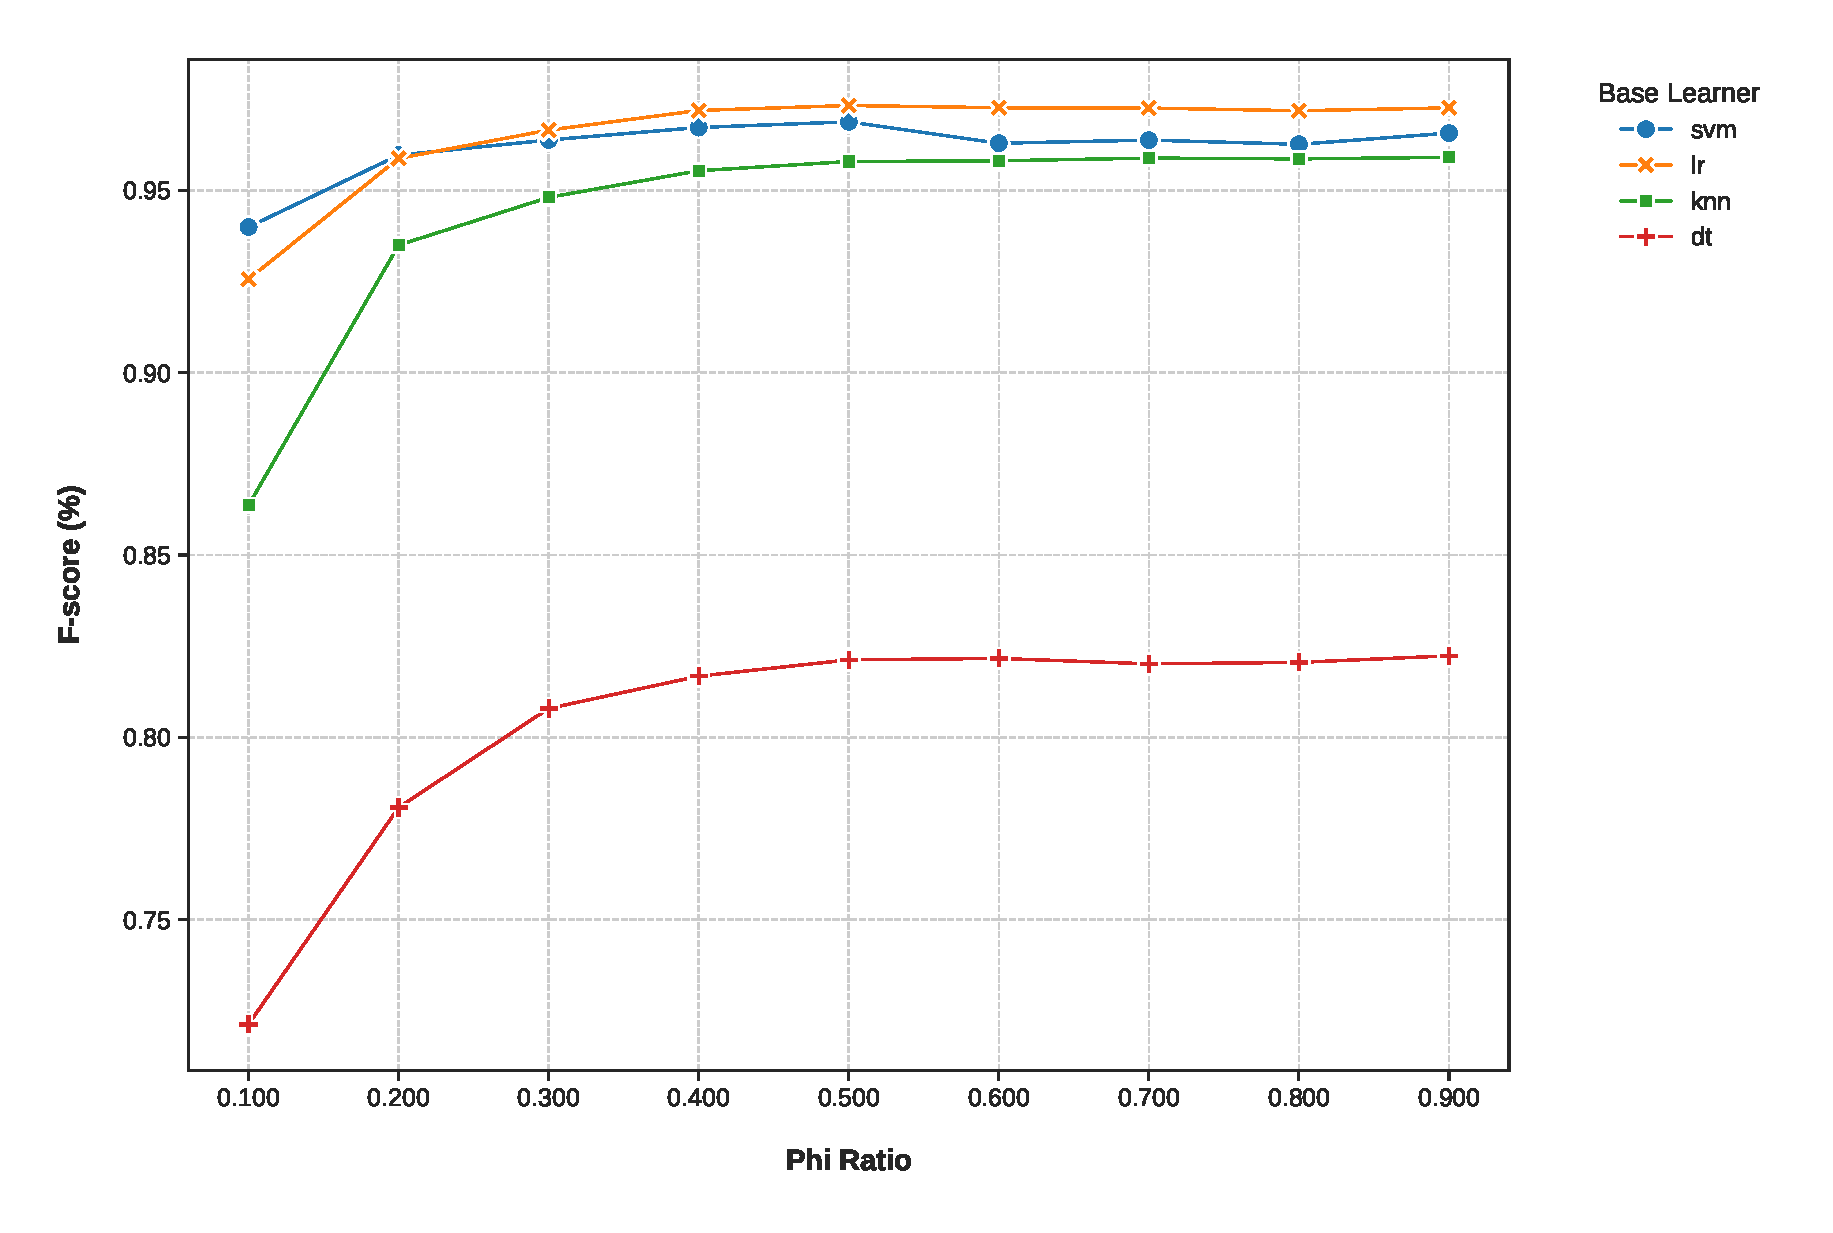
\includegraphics[width=0.7\linewidth]{fscore_vs_phi}
		\caption{F-score vs Sampling Ratio for Density ensemble method}
		\label{fig:fscore_vs_clusters}
	\end{figure*}
	
	\begin{figure*}[t!]
		\centering
		
\includegraphics[width=0.7\linewidth]{fscore_vs_clusters}
		\caption{F-score vs Number of Clusters for Density ensemble method}
		\label{fig:fscore_vs_phi}
	\end{figure*}
	
	Figure \ref{fig:boxplot_comparison} provides a visual representation of the distribution of scores for
	each ensemble method and base learner combination. This figure reinforces
	the tabulated results, highlighting the overall superior performance of the
	DensityE and DistE methods. The variability in scores is also depicted,
	with DensityE and DistE showing tighter distributions compared to AvgE
	and MaxE. Notably, the single SVM model achieves a high and consistent
	performance, underscoring the robustness of SVM as a standalone model.
	
	\begin{figure*}[!t]
		\centering
		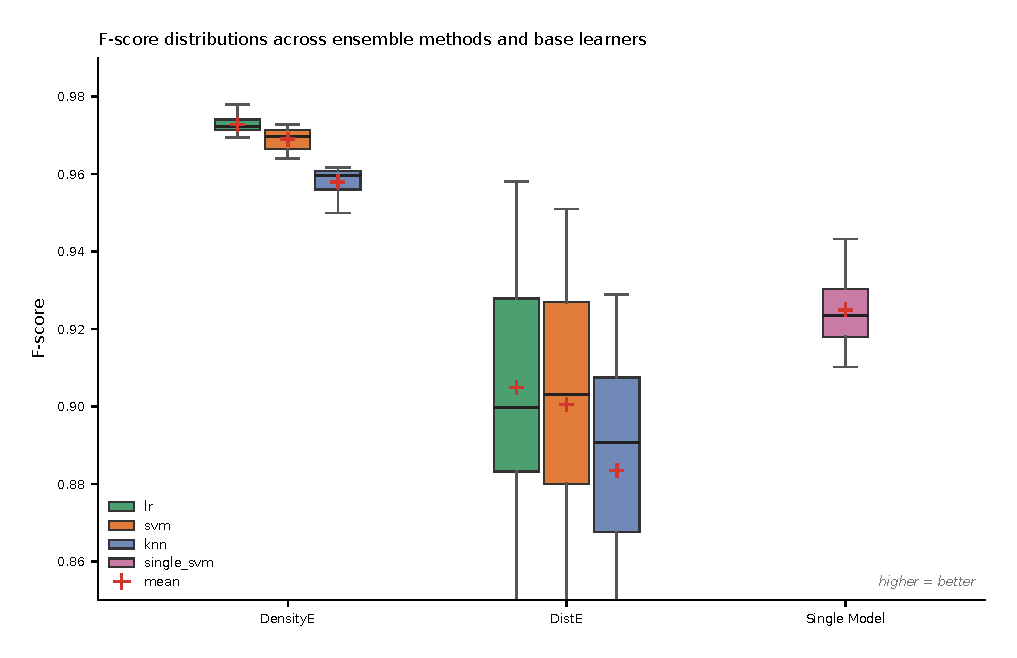
\includegraphics[width=0.7\linewidth]{boxplot_comparison}
		\caption{Comparison of F-score Distributions Across Different Ensemble Methods and Base Learners}
		\label{fig:boxplot_comparison}
	\end{figure*}
	
	\section{Discussion}
	
	\noindent The results unequivocally indicate that the DensityE ensemble method offers superior performance compared to other ensemble methods, particularly when logistic regression and support vector machine are utilized as base learners. This finding underscores the efficacy of DensityE’s approach in leveraging the strengths of diverse base learners and effectively managing their combined output. The superior performance of logistic regression and support vector machine base learners can be attributed to their robustness and strong generalization capabilities, especially when applied to data with complex underlying distributions.
	
	The comparative analysis across different base learners highlights the critical role of base learner selection in ensemble methods. While linear models
	like logistic regression and support vector machine benefit significantly from
	the ensemble approach, non-linear models such as k-nearest neighbors and
	decision trees show relatively lower performance. This disparity may be due
	to the inherent differences in how these models handle data complexity and
	variability.
	
	The insights gained from Figures 1 and 2 provide a deeper understanding
	of ensemble dynamics. Increasing the number of clusters generally leads
	to better performance, but the benefits diminish beyond a certain point.
	Similarly, a higher sampling ratio enhances the F-score, emphasizing the
	value of larger training samples for achieving higher accuracy.
	
	In conclusion, the DensityE ensemble method, particularly when paired
	with logistic regression and support vector machine base learners, demonstrates the most promising performance. Future research could explore the
	integration of more sophisticated base learners and the application of these
	ensemble methods to various types of datasets to further validate their robustness and generalizability. Additionally, investigating the effects of varying other parameters within the DensityE method may yield further performance improvements and insights.
	
	
	\section{Conclusion}
	\noindent
	
	In this paper, we introduced the Density-Based Dynamic Ensemble Learning Algorithm using Gaussian Mixture Models (DDEL-GMM), a novel framework specifically engineered to enhance the personalization of predictions in complex data environments. The core challenge addressed is the limitation of traditional models in adapting to the unique characteristics of individual data points. DDEL-GMM tackles this by employing a sophisticated two-stage process. First, it uses Gaussian Mixture Models to partition the data into nuanced, overlapping clusters, capturing underlying data structures more effectively than methods based on rigid partitioning. This allows for the training of highly specialized base classifiers. Second, its density-based dynamic selection mechanism creates a bespoke, weighted ensemble for each individual test instance, ensuring that the final prediction is highly personalized and context-aware.
	
	Our experimental evaluation confirmed the superior performance of this personalized approach. DDEL-GMM, particularly when paired with Logistic Regression and Support Vector Machine base learners, significantly outperformed other ensemble strategies. Crucially, it addresses the key limitations of prior work such as the DELAK model. While DELAK utilizes K-means, which struggles with non-spherical data distributions, DDEL-GMM's use of GMMs allows for a more flexible and accurate modeling of complex data structures. This leads to a more effective specialization of base learners and, ultimately, more precise predictions. The density-based selection further refines the model's competence assessment beyond simple distance metrics, enhancing its robustness and accuracy.
	
	The findings establish DDEL-GMM as a powerful solution for classification tasks where personalization is paramount. The primary contribution of this work is a robust framework that advances the state-of-the-art in dynamic ensemble learning by delivering more accurate, reliable, and highly personalized predictive analytics.
	
	Future research will aim to build upon this foundation. We intend to explore the integration of more diverse and complex base learners and to test the framework’s generalizability across various domains where personalized modeling is critical, such as personalized medicine and financial risk assessment. Further investigation into optimizing the GMM clustering phase and adapting the framework for real-time data streams will also be key areas of focus.
	
	\bibliographystyle{IEEEtran}
	\bibliography{references}
	
	%\begin{IEEEbiography}[{\includegraphics[width=1in,height=1.25in,clip,keepaspectratio]{fig1.png}}]{IEEE Publications Technology Team}
	%In this paragraph you can place your educational, professional background and research and other interests.\end{IEEEbiography}


\end{document}